
%% bare_conf.tex
%% V1.3
%% 2007/01/11
%% by Michael Shell
%% See:
%% http://www.michaelshell.org/
%% for current contact information.
%%
%% This is a skeleton file demonstrating the use of IEEEtran.cls
%% (requires IEEEtran.cls version 1.7 or later) with an IEEE conference paper.
%%
%% Support sites:
%% http://www.michaelshell.org/tex/ieeetran/
%% http://www.ctan.org/tex-archive/macros/latex/contrib/IEEEtran/
%% and
%% http://www.ieee.org/

%%*************************************************************************
%% Legal Notice:
%% This code is offered as-is without any warranty either expressed or
%% implied; without even the implied warranty of MERCHANTABILITY or
%% FITNESS FOR A PARTICULAR PURPOSE! 
%% User assumes all risk.
%% In no event shall IEEE or any contributor to this code be liable for
%% any damages or losses, including, but not limited to, incidental,
%% consequential, or any other damages, resulting from the use or misuse
%% of any information contained here.
%%
%% All comments are the opinions of their respective authors and are not
%% necessarily endorsed by the IEEE.
%%
%% This work is distributed under the LaTeX Project Public License (LPPL)
%% ( http://www.latex-project.org/ ) version 1.3, and may be freely used,
%% distributed and modified. A copy of the LPPL, version 1.3, is included
%% in the base LaTeX documentation of all distributions of LaTeX released
%% 2003/12/01 or later.
%% Retain all contribution notices and credits.
%% ** Modified files should be clearly indicated as such, including  **
%% ** renaming them and changing author support contact information. **
%%
%% File list of work: IEEEtran.cls, IEEEtran_HOWTO.pdf, bare_adv.tex,
%%                    bare_conf.tex, bare_jrnl.tex, bare_jrnl_compsoc.tex
%%*************************************************************************

% *** Authors should verify (and, if needed, correct) their LaTeX system  ***
% *** with the testflow diagnostic prior to trusting their LaTeX platform ***
% *** with production work. IEEE's font choices can trigger bugs that do  ***
% *** not appear when using other class files.                            ***
% The testflow support page is at:
% http://www.michaelshell.org/tex/testflow/



% Note that the a4paper option is mainly intended so that authors in
% countries using A4 can easily print to A4 and see how their papers will
% look in print - the typesetting of the document will not typically be
% affected with changes in paper size (but the bottom and side margins will).
% Use the testflow package mentioned above to verify correct handling of
% both paper sizes by the user's LaTeX system.
%
% Also note that the "draftcls" or "draftclsnofoot", not "draft", option
% should be used if it is desired that the figures are to be displayed in
% draft mode.
%
\documentclass[conference]{IEEEtran}
% Add the compsoc option for Computer Society conferences.
%
% If IEEEtran.cls has not been installed into the LaTeX system files,
% manually specify the path to it like:
% \documentclass[conference]{../sty/IEEEtran}





% Some very useful LaTeX packages include:
% (uncomment the ones you want to load)


% *** MISC UTILITY PACKAGES ***
%
%\usepackage{ifpdf}
% Heiko Oberdiek's ifpdf.sty is very useful if you need conditional
% compilation based on whether the output is pdf or dvi.
% usage:
% \ifpdf
%   % pdf code
% \else
%   % dvi code
% \fi
% The latest version of ifpdf.sty can be obtained from:
% http://www.ctan.org/tex-archive/macros/latex/contrib/oberdiek/
% Also, note that IEEEtran.cls V1.7 and later provides a builtin
% \ifCLASSINFOpdf conditional that works the same way.
% When switching from latex to pdflatex and vice-versa, the compiler may
% have to be run twice to clear warning/error messages.






% *** CITATION PACKAGES ***
%
%\usepackage{cite}
% cite.sty was written by Donald Arseneau
% V1.6 and later of IEEEtran pre-defines the format of the cite.sty package
% \cite{} output to follow that of IEEE. Loading the cite package will
% result in citation numbers being automatically sorted and properly
% "compressed/ranged". e.g., [1], [9], [2], [7], [5], [6] without using
% cite.sty will become [1], [2], [5]--[7], [9] using cite.sty. cite.sty's
% \cite will automatically add leading space, if needed. Use cite.sty's
% noadjust option (cite.sty V3.8 and later) if you want to turn this off.
% cite.sty is already installed on most LaTeX systems. Be sure and use
% version 4.0 (2003-05-27) and later if using hyperref.sty. cite.sty does
% not currently provide for hyperlinked citations.
% The latest version can be obtained at:
% http://www.ctan.org/tex-archive/macros/latex/contrib/cite/
% The documentation is contained in the cite.sty file itself.






% *** GRAPHICS RELATED PACKAGES ***
%
\ifCLASSINFOpdf
   \usepackage[pdftex]{graphicx}
  % declare the path(s) where your graphic files are
  % \graphicspath{{../pdf/}{../jpeg/}}
  % and their extensions so you won't have to specify these with
  % every instance of \includegraphics
  % \DeclareGraphicsExtensions{.pdf,.jpeg,.png}
\else
  % or other class option (dvipsone, dvipdf, if not using dvips). graphicx
  % will default to the driver specified in the system graphics.cfg if no
  % driver is specified.
   \usepackage[dvips]{graphicx}
  % declare the path(s) where your graphic files are
  % \graphicspath{{../eps/}}
  % and their extensions so you won't have to specify these with
  % every instance of \includegraphics
  % \DeclareGraphicsExtensions{.eps}
\fi
% graphicx was written by David Carlisle and Sebastian Rahtz. It is
% required if you want graphics, photos, etc. graphicx.sty is already
% installed on most LaTeX systems. The latest version and documentation can
% be obtained at: 
% http://www.ctan.org/tex-archive/macros/latex/required/graphics/
% Another good source of documentation is "Using Imported Graphics in
% LaTeX2e" by Keith Reckdahl which can be found as epslatex.ps or
% epslatex.pdf at: http://www.ctan.org/tex-archive/info/
%
% latex, and pdflatex in dvi mode, support graphics in encapsulated
% postscript (.eps) format. pdflatex in pdf mode supports graphics
% in .pdf, .jpeg, .png and .mps (metapost) formats. Users should ensure
% that all non-photo figures use a vector format (.eps, .pdf, .mps) and
% not a bitmapped formats (.jpeg, .png). IEEE frowns on bitmapped formats
% which can result in "jaggedy"/blurry rendering of lines and letters as
% well as large increases in file sizes.
%
% You can find documentation about the pdfTeX application at:
% http://www.tug.org/applications/pdftex





% *** MATH PACKAGES ***
%
\usepackage[cmex10]{amsmath}
% A popular package from the American Mathematical Society that provides
% many useful and powerful commands for dealing with mathematics. If using
% it, be sure to load this package with the cmex10 option to ensure that
% only type 1 fonts will utilized at all point sizes. Without this option,
% it is possible that some math symbols, particularly those within
% footnotes, will be rendered in bitmap form which will result in a
% document that can not be IEEE Xplore compliant!
%
% Also, note that the amsmath package sets \interdisplaylinepenalty to 10000
% thus preventing page breaks from occurring within multiline equations. Use:
%\interdisplaylinepenalty=2500
% after loading amsmath to restore such page breaks as IEEEtran.cls normally
% does. amsmath.sty is already installed on most LaTeX systems. The latest
% version and documentation can be obtained at:
% http://www.ctan.org/tex-archive/macros/latex/required/amslatex/math/





% *** SPECIALIZED LIST PACKAGES ***
%
\usepackage{algorithmic}
% algorithmic.sty was written by Peter Williams and Rogerio Brito.
% This package provides an algorithmic environment fo describing algorithms.
% You can use the algorithmic environment in-text or within a figure
% environment to provide for a floating algorithm. Do NOT use the algorithm
% floating environment provided by algorithm.sty (by the same authors) or
% algorithm2e.sty (by Christophe Fiorio) as IEEE does not use dedicated
% algorithm float types and packages that provide these will not provide
% correct IEEE style captions. The latest version and documentation of
% algorithmic.sty can be obtained at:
% http://www.ctan.org/tex-archive/macros/latex/contrib/algorithms/
% There is also a support site at:
% http://algorithms.berlios.de/index.html
% Also of interest may be the (relatively newer and more customizable)
% algorithmicx.sty package by Szasz Janos:
% http://www.ctan.org/tex-archive/macros/latex/contrib/algorithmicx/




% *** ALIGNMENT PACKAGES ***
%
%\usepackage{array}
% Frank Mittelbach's and David Carlisle's array.sty patches and improves
% the standard LaTeX2e array and tabular environments to provide better
% appearance and additional user controls. As the default LaTeX2e table
% generation code is lacking to the point of almost being broken with
% respect to the quality of the end results, all users are strongly
% advised to use an enhanced (at the very least that provided by array.sty)
% set of table tools. array.sty is already installed on most systems. The
% latest version and documentation can be obtained at:
% http://www.ctan.org/tex-archive/macros/latex/required/tools/


%\usepackage{mdwmath}
%\usepackage{mdwtab}
% Also highly recommended is Mark Wooding's extremely powerful MDW tools,
% especially mdwmath.sty and mdwtab.sty which are used to format equations
% and tables, respectively. The MDWtools set is already installed on most
% LaTeX systems. The lastest version and documentation is available at:
% http://www.ctan.org/tex-archive/macros/latex/contrib/mdwtools/


% IEEEtran contains the IEEEeqnarray family of commands that can be used to
% generate multiline equations as well as matrices, tables, etc., of high
% quality.


%\usepackage{eqparbox}
% Also of notable interest is Scott Pakin's eqparbox package for creating
% (automatically sized) equal width boxes - aka "natural width parboxes".
% Available at:
% http://www.ctan.org/tex-archive/macros/latex/contrib/eqparbox/





% *** SUBFIGURE PACKAGES ***
%\usepackage[tight,footnotesize]{subfigure}
% subfigure.sty was written by Steven Douglas Cochran. This package makes it
% easy to put subfigures in your figures. e.g., "Figure 1a and 1b". For IEEE
% work, it is a good idea to load it with the tight package option to reduce
% the amount of white space around the subfigures. subfigure.sty is already
% installed on most LaTeX systems. The latest version and documentation can
% be obtained at:
% http://www.ctan.org/tex-archive/obsolete/macros/latex/contrib/subfigure/
% subfigure.sty has been superceeded by subfig.sty.



%\usepackage[caption=false]{caption}
%\usepackage[font=footnotesize]{subfig}
% subfig.sty, also written by Steven Douglas Cochran, is the modern
% replacement for subfigure.sty. However, subfig.sty requires and
% automatically loads Axel Sommerfeldt's caption.sty which will override
% IEEEtran.cls handling of captions and this will result in nonIEEE style
% figure/table captions. To prevent this problem, be sure and preload
% caption.sty with its "caption=false" package option. This is will preserve
% IEEEtran.cls handing of captions. Version 1.3 (2005/06/28) and later 
% (recommended due to many improvements over 1.2) of subfig.sty supports
% the caption=false option directly:
%\usepackage[caption=false,font=footnotesize]{subfig}
%
% The latest version and documentation can be obtained at:
% http://www.ctan.org/tex-archive/macros/latex/contrib/subfig/
% The latest version and documentation of caption.sty can be obtained at:
% http://www.ctan.org/tex-archive/macros/latex/contrib/caption/




% *** FLOAT PACKAGES ***
%
%\usepackage{fixltx2e}
% fixltx2e, the successor to the earlier fix2col.sty, was written by
% Frank Mittelbach and David Carlisle. This package corrects a few problems
% in the LaTeX2e kernel, the most notable of which is that in current
% LaTeX2e releases, the ordering of single and double column floats is not
% guaranteed to be preserved. Thus, an unpatched LaTeX2e can allow a
% single column figure to be placed prior to an earlier double column
% figure. The latest version and documentation can be found at:
% http://www.ctan.org/tex-archive/macros/latex/base/



%\usepackage{stfloats}
% stfloats.sty was written by Sigitas Tolusis. This package gives LaTeX2e
% the ability to do double column floats at the bottom of the page as well
% as the top. (e.g., "\begin{figure*}[!b]" is not normally possible in
% LaTeX2e). It also provides a command:
%\fnbelowfloat
% to enable the placement of footnotes below bottom floats (the standard
% LaTeX2e kernel puts them above bottom floats). This is an invasive package
% which rewrites many portions of the LaTeX2e float routines. It may not work
% with other packages that modify the LaTeX2e float routines. The latest
% version and documentation can be obtained at:
% http://www.ctan.org/tex-archive/macros/latex/contrib/sttools/
% Documentation is contained in the stfloats.sty comments as well as in the
% presfull.pdf file. Do not use the stfloats baselinefloat ability as IEEE
% does not allow \baselineskip to stretch. Authors submitting work to the
% IEEE should note that IEEE rarely uses double column equations and
% that authors should try to avoid such use. Do not be tempted to use the
% cuted.sty or midfloat.sty packages (also by Sigitas Tolusis) as IEEE does
% not format its papers in such ways.





% *** PDF, URL AND HYPERLINK PACKAGES ***
%
%\usepackage{url}
% url.sty was written by Donald Arseneau. It provides better support for
% handling and breaking URLs. url.sty is already installed on most LaTeX
% systems. The latest version can be obtained at:
% http://www.ctan.org/tex-archive/macros/latex/contrib/misc/
% Read the url.sty source comments for usage information. Basically,
% \url{my_url_here}.





% *** Do not adjust lengths that control margins, column widths, etc. ***
% *** Do not use packages that alter fonts (such as pslatex).         ***
% There should be no need to do such things with IEEEtran.cls V1.6 and later.
% (Unless specifically asked to do so by the journal or conference you plan
% to submit to, of course. )



\usepackage{alltt}

\usepackage{algorithm}
\usepackage{bbold}

\usepackage{pstricks-add}

\renewcommand{\algorithmicrequire}{\textbf{Input:}}
\newtheorem{theorem}{Theorem}[section]

\newtheorem{definition}{Definition}
\newtheorem{lemma}[definition]{Lemma}
% correct bad hyphenation here
\hyphenation{op-tical net-works semi-conduc-tor}


\begin{document}
%
% paper title
% can use linebreaks \\ within to get better formatting as desired
\title{A Methodology for Comparing and Creating Community Metrics}


% author names and affiliations
% use a multiple column layout for up to three different
% affiliations
\author{\IEEEauthorblockN{June Andrews}
\IEEEauthorblockA{Center for Applied Math\\
Cornell University\\
Ithaca, NY 14853\\
http://www.cam.cornell.edu/~jandrews}
\and
\IEEEauthorblockN{John Hopcroft}
\IEEEauthorblockA{Computer Science Dept\\
Cornell University\\
Ithaca, NY 14853\\
Email:jeh@cs.cornell.edu}
}

% conference papers do not typically use \thanks and this command
% is locked out in conference mode. If really needed, such as for
% the acknowledgment of grants, issue a \IEEEoverridecommandlockouts
% after \documentclass

% for over three affiliations, or if they all won't fit within the width
% of the page, use this alternative format:
% 
%\author{\IEEEauthorblockN{Michael Shell\IEEEauthorrefmark{1},
%Homer Simpson\IEEEauthorrefmark{2},
%James Kirk\IEEEauthorrefmark{3}, 
%Montgomery Scott\IEEEauthorrefmark{3} and
%Eldon Tyrell\IEEEauthorrefmark{4}}
%\IEEEauthorblockA{\IEEEauthorrefmark{1}School of Electrical and Computer Engineering\\
%Georgia Institute of Technology,
%Atlanta, Georgia 30332--0250\\ Email: see http://www.michaelshell.org/contact.html}
%\IEEEauthorblockA{\IEEEauthorrefmark{2}Twentieth Century Fox, Springfield, USA\\
%Email: homer@thesimpsons.com}
%\IEEEauthorblockA{\IEEEauthorrefmark{3}Starfleet Academy, San Francisco, California 96678-2391\\
%Telephone: (800) 555--1212, Fax: (888) 555--1212}
%\IEEEauthorblockA{\IEEEauthorrefmark{4}Tyrell Inc., 123 Replicant Street, Los Angeles, California 90210--4321}}




% use for special paper notices
%\IEEEspecialpapernotice{(Invited Paper)}




% make the title area
\maketitle


\begin{abstract}
%\boldmath
Community detection is used to understand the structure of large networks and
their inner workings. It decomposes the network into a set of well-connected
subgraphs, each of which is deemed a community. Complications arise in defining
well-connected. Stemming from a variety of intuitions, several definitions have
arisen. Two prominent definitions are: modularity \cite{modularity}, based off of an expected
subgraph's density, and conductance\cite{conductance}, based off of the ratio of external edges
to all edges of a subgraph. The communities determined by each definition are
different and have only been compared through experimental methods. 

We present a framework that allows theoretical comparison of metric based
community detection methods. We first parametrize metrics in terms of internal
density and external sparsity of subgraphs. Once in this space, we use level
sets to make clear what types of communities a metric will return. Our results
support and expand upon published experimental results. 

From this framework a new family of metrics becomes apparent. The Louvain
Algorithm\cite{louvain} is easily adapted to optimize for this new family of metrics and to
return meaningful overlapping communities. We confirm our theoretical results
with experiments on selected large networks and assert our improvement over
modularity within our framework.

\end{abstract}

Keywords:
Community Detection, Community Metrics, Networks
% IEEEtran.cls defaults to using nonbold math in the Abstract.
% This preserves the distinction between vectors and scalars. However,
% if the conference you are submitting to favors bold math in the abstract,
% then you can use LaTeX's standard command \boldmath at the very start
% of the abstract to achieve this. Many IEEE journals/conferences frown on
% math in the abstract anyway.

% no keywords



% For peer review papers, you can put extra information on the cover
% page as needed:
% \ifCLASSOPTIONpeerreview
% \begin{center} \bfseries EDICS Category: 3-BBND \end{center}
% \fi
%
% For peerreview papers, this IEEEtran command inserts a page break and
% creates the second title. It will be ignored for other modes.
\IEEEpeerreviewmaketitle


\section{Introduction}

Community detection allows us to decompose large networks into communities.  The uses of these communities are for classifying nodes[].  A natural byproduct of decomposing large networks is to measure how well a decomposition describes a network.  Applications, desire decompositions that select subsets of nodes with good internal connectivity.  In a social graph, good connectivity of a subset of nodes indicates a group of friends, colleagues, or some common collective association between the people involved.  In a citation network, good connectivity indicates a general topic shared between the papers. 

The quality of a network decomposition in communities, or the strength of meaning of one network, have been analyzed based on metrics to measure their internal connectivity.  Several metrics exist.  The metrics are derived from intuitive definitions of what a community should be.  Empirical comparisons of the metrics have been made.  Empirical comparison to date have taken sets of networks, applied algorithms to maximize the metrics, and compared the communities on another criteria.  In particular, Leskovec et al\cite{leskovec:empirical} compare detected communities with conductance, modularity ratio, and several other metrics.  Leskovec et al reach conclusions about what types of communities each metric favors on given networks.  We seek to expand the conclusions that can be reached by comparing metrics in a theoretical environment.  We test the results on known data sets.


We present a simple framework to allow comparison of metrics before implementation.  This framework reveals a methodology for creating new metrics, should an application demand.  We provide a basic metric and test it theoretically and with specific implementations.  We adapt the dendogram based on the Louvain algorithm \cite{louvain}, to quickly implement a metric maximization of these new metrics.

As applications for community metrics expand, we recommend this framework for adapting algorithms to application specific problems.  Certain problems have more sensitivity or less space.  Our framework allows customization to the needs of sensitivity to dense communities, encompassing all edges of the graph, and space to describe all communities.

This paper lays out community definitions for comparison of single communities and network covering community decompositions.  Depending on the questions asked metrics for either case may be more appropriate.  Our framework requires little adaptation between the two cases and produces new metrics for both.  To start from a problem everyone is familiar with we use the Karate Club and Football Game network as our small scale network examples and the Physics Citation Archive as a larger scale network example.  Maximizing the new metrics runs in time proportional to runtimes for modularity maximization.  Hence, maximizing the new metric can be applied to larger networks.

Our notation throughout the paper will be conventional:
\begin{center}
\begin{tabular}{|c|c|}
\hline  Network & $G(V, E)$\\ \hline 
Nodes & $u,v \in V$ \\ \hline
Weighted Edges & $w: V^2 \rightarrow \mathbb{R}_+ \leq 1$ \\ \hline
Community & $C \subseteq V$ \\ \hline
Size of $C$ & $|C| = k |V|$ \\ \hline
Set of Communities & $S = \{C_1, C_2, \dots, C_n\}$ \\ \hline
\end{tabular}
\end{center}
We use the convention that all edges are positively weighted, with a maximum weight of $1$, and all possible edges exist.  If an edge does not exist in the network, we add it with $0$ weight for ease of mathematical notation.

\section{Metrics for Single Communities}

Community definitions for single communities are metrics that determine whether or not a subset of node of the graph are appropriately well connected to each other and sparsely connected to the rest of the graph.  We cover six popular metrics of single communities.
There exist more definitions of single communities: $(\alpha, \beta)$, out degree fraction metrics, and variations of those.  However, those definitions are not based on internal and external density, but rather on worst case analysis.  We only consider the majority of definitions that are based on internal and external density of the entire community.

For a single community the accepted ideal community is a clique of nodes disconnected from the rest of the graph.  This description depends on two parameters internal density and external sparsity.  We formalize internal and external density.
\begin{definition}[Internal Density]
  \begin{align*}
   I(C) &=  \frac{\sum_{u \in C}\sum_{v \in C} w(u,v)}{|C|(|C| - 1)} 
\end{align*}
\end{definition}
\begin{definition}[External Density]
\begin{align*}
  E(C) &=\frac{\sum_{u \in C}\sum_{v \notin C} w(u,v)}{|C|(|V| - |C|)}.
  \end{align*}
\end{definition}
There are other representations of $I(C)$ and $E(C)$ that vary the $|C|$ and $|V| - |C|$ terms.  The analysis and conclusions that follow are not sensitive those variations..  We can now dictate what the ideal community is mathematically:
\begin{definition}[Ideal Single Community]
 A community, $C$, is ideal if it is an isolated clique and has the following properties:
  \begin{align*}
   I(C) &= 1 \\
   E(C) &= 0.
  \end{align*}
\end{definition}


\subsection{Specific Metrics}

We cover six metrics for single communities:
\begin{itemize}[]
 \item {\sc Conductance}: the probability that a step in a random walk will leave the community \cite{conductance}.
 \item {\sc Cut Ratio}: the fraction of existing to possible edges leaving the community \cite{cut_ratio}.
 \item {\sc Edges Cuts}: the number of edges connecting the community to the rest of the graph \cite{edges_cut}.
  \item {\sc Expansion}: the average number of edges leaving the community per node \cite{expansion}.
  \item {\sc Internal Density}: internal density of the community \cite{i_density}.
  \item {\sc Volume}: the total degree of nodes within the community \cite{volume}.
\end{itemize}



\subsection{Parameterizations}
We can now parameterize the described metrics in terms of internal and external density.  We use the definitions from the previous section, the approximations $|C| \approx |C| - 1$, and the variable $k$ to simplify $|C|  = k |V|$.  Hence we can put all previously described metrics in terms of $I(C)$, $E(C)$, $|C|$, $|V|$, and $k$.

\begin{align*}
 \text{\sc Conductance}(C) &= \frac{(1-k)E(C)}{kI(C) + (1-k)E(C)} \\
& \\
 \text{\sc Cut Ratio} &=  k(1-k)|V|^2E(C)\\
& \\
 \text{\sc Edge Cuts} &= E(C)\\
& \\
\text{\sc Expansion} &= (1- k)|V|  E(C) \\
& \\
 \text{\sc Internal Density} &=  1 - I(C) \\
& \\
 \text{\sc Volume} &= |C|^2I(C) + (1-k)|C||V|E(C)
\end{align*}

Our first observation is that not all metrics are functions of both $I(C)$ and $E(C)$.  We address the implications of a metric defined over only $I(C)$ or $E(C)$ in later sections.

\subsection{Greedy Optimization}
We now use a simple greedy algorithm for each of these metrics to observe what types of communities optimize each metric. The algorithm is:
\begin{algorithm}                      		% enter the algorithm environment
\caption{Greedy Single Community Metric Optimization}     	% give the algorithm a caption
\label{alg1}                           		% and a label for \ref{} commands later in the document
\begin{algorithmic}                    	% enter the algorithmic environment
\REQUIRE $C$, $G=(V,E)$, and {\sc Metric}
\STATE $inc = 1.$
\WHILE{$inc \geq 0$ and $C \neq V$}
\STATE Let $u \in V$ maximize {\sc Metric}$(C \cup u)$.
\STATE $inc =$ {\sc Metric}$(C \cup u) - $  {\sc Metric}$(C)$
\STATE Augment $C$ by $u$
\ENDWHILE
\end{algorithmic}
\end{algorithm}

Some metrics require minimization rather than maximization, this algorithm is easily adapted accordingly.

For each metric we start the algorithm with a simple subset of two connected nodes and track the communities that result in improvements, according to a given metric.  As the algorithm expands the community, the metric determines which node is optimal at each step.  We record this better community and for each metric, $M$, get a set of $C_1, C_2, \dots C_n$, such that the metric is increasing $M(C_i) < M(C_{i+1})$.  While this is not an encompassing algorithm that checks for all communities, it will reveal a metric's biasenesses toward communities of certain $I(C)$, $E(C)$, values.

We apply the greedy algorithm to the well-known Zachary's Karate Club[] and the American College Football Game[] data sets and obtain {\it Fig.  \ref{fig_single_metrics}}.
\begin{figure}[!h]
\centering
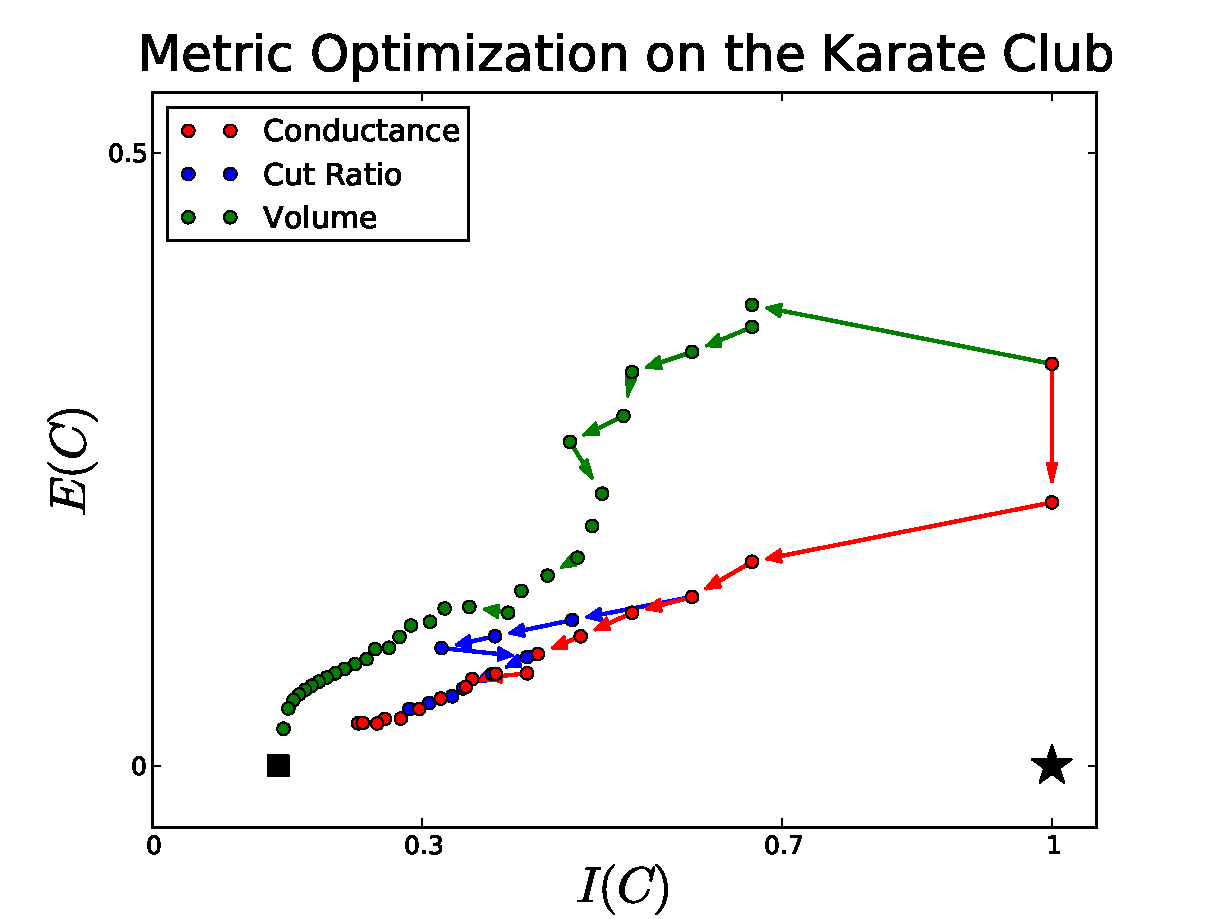
\includegraphics[width=3in]{Figures/karate_metrics}
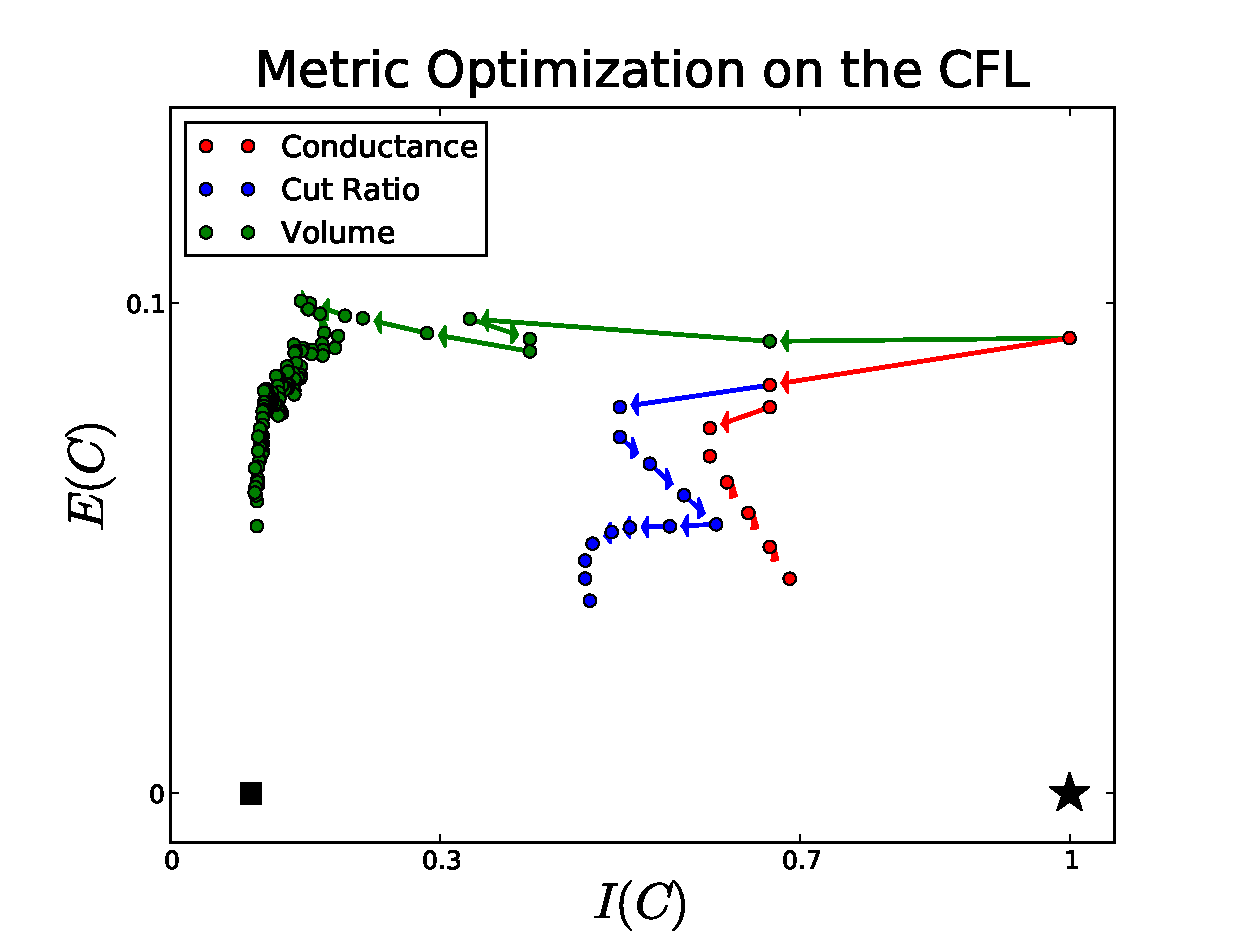
\includegraphics[width=3in]{Figures/football_metrics}
\caption{Seeding the greedy algorithm with two connected nodes, we track the communities produced by optimizing each metric in the $I, E$ plane.  The black star is the definition of an ideal community and the black square is the $I,E$ value of a community encompassing the entire graph.}
\label{fig_single_metrics}
\end{figure}
The metrics edge cuts, expansion, and internal density are not included as their paths overlaps other metric's paths.  In the Karate Club optimizing conductance, cut ratio, and volume leads to nearly encompassing the entire graph.  In the College Football Leagues the metric's behavior is a little less predictable.


\subsection{Level Sets}
So far we have parameterized the metrics in terms of internal and external density and shown that their optimization appears sporadic and suboptimal at times.  However, the metrics are being optimized.  What has not been taken into account is how the metrics optimize over the $I,E$ plane.  We can visualize their optimizations by calculating the value of the metric for all points of the $I,E$ plane and graphing the contour curves, or level sets[].  In level set figures, any two points in the $I,E$ plane connected by a curve have the same metric value. We now show how the metrics optimize in regard to the $I,E$ plane and show that level sets explain the greedy optimization's path through the $I,E$ plane.

\subsubsection{Conductance Level Sets}
For conductance the level sets are rays radiating from $(I, E) = (0, 0)$, see {\it Fig. \ref{fig_conductance_karate}}.  As the rays become closer to horizontal, $E = 0$, conductance becomes optimal.  Hence, no matter the data set, conductance desires communities with $I,E$ values closer to $(I,E) = (x, 0)$, for any arbitrary $I(C) = x$.  Including more nodes that continually increase $I(C)$ is rare in networks and much more common is decreasing $E(C)$ by encompassing more of the graph.  Since, conductance is fairly, unresponsive to changes in $I(C)$, optimizing conductance results decreasing $E(C)$ as much as possible.  How much conductance is biased towards small improvements in $E(C)$ verse large improvements in $I(C)$ depends on where in the $I,E$ domain the seed communities originate.   In the College Football League, the seed community begins a portion of the domain where improvements in $I$ and $E$ are balanced.  For Zarchary's Karate Club, the seed community quickly falls into a portion of the $I,E$ domain where small and easy improvements in $E$ benefit conductance more than large and hard changes in $I$.

\begin{figure}[!h]
\centering
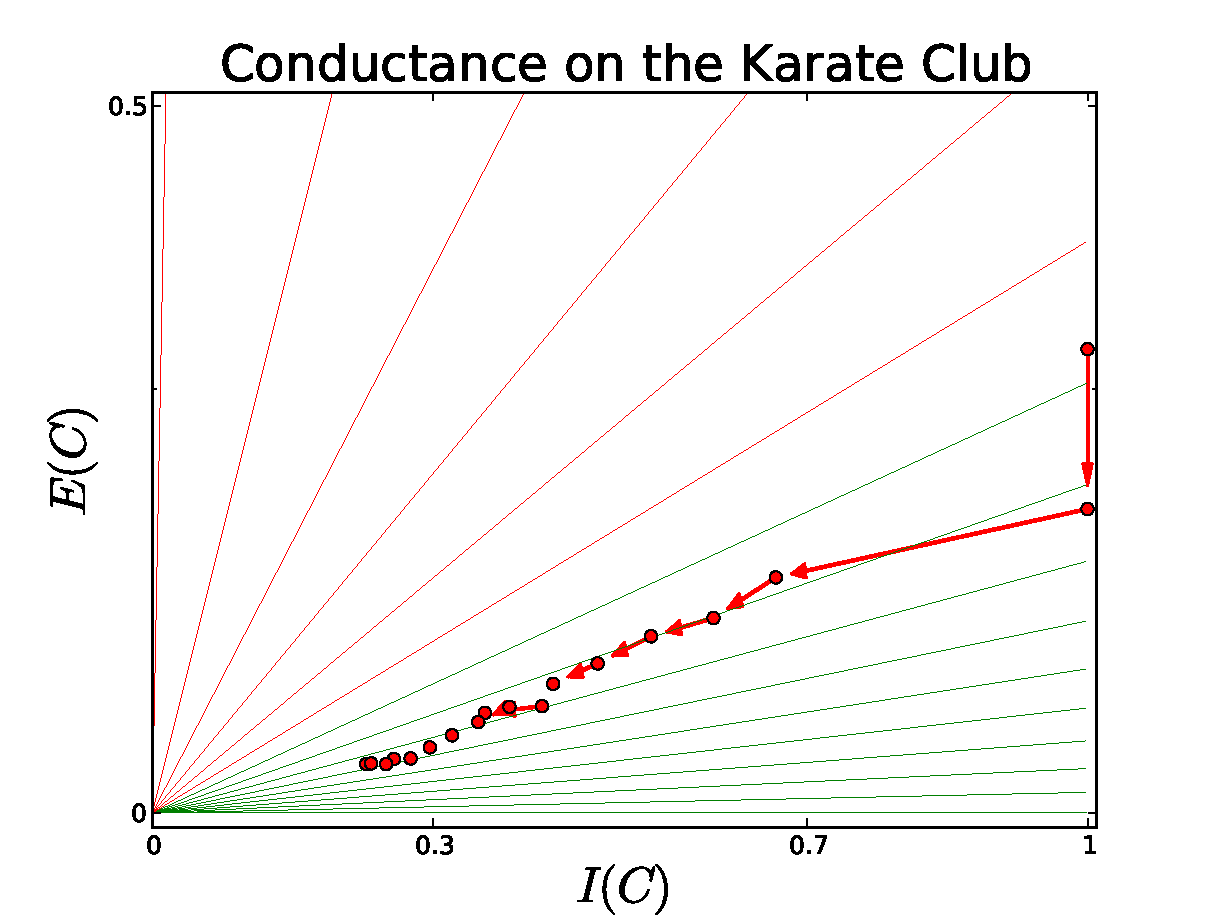
\includegraphics[width=3in]{Figures/karate_conductance}
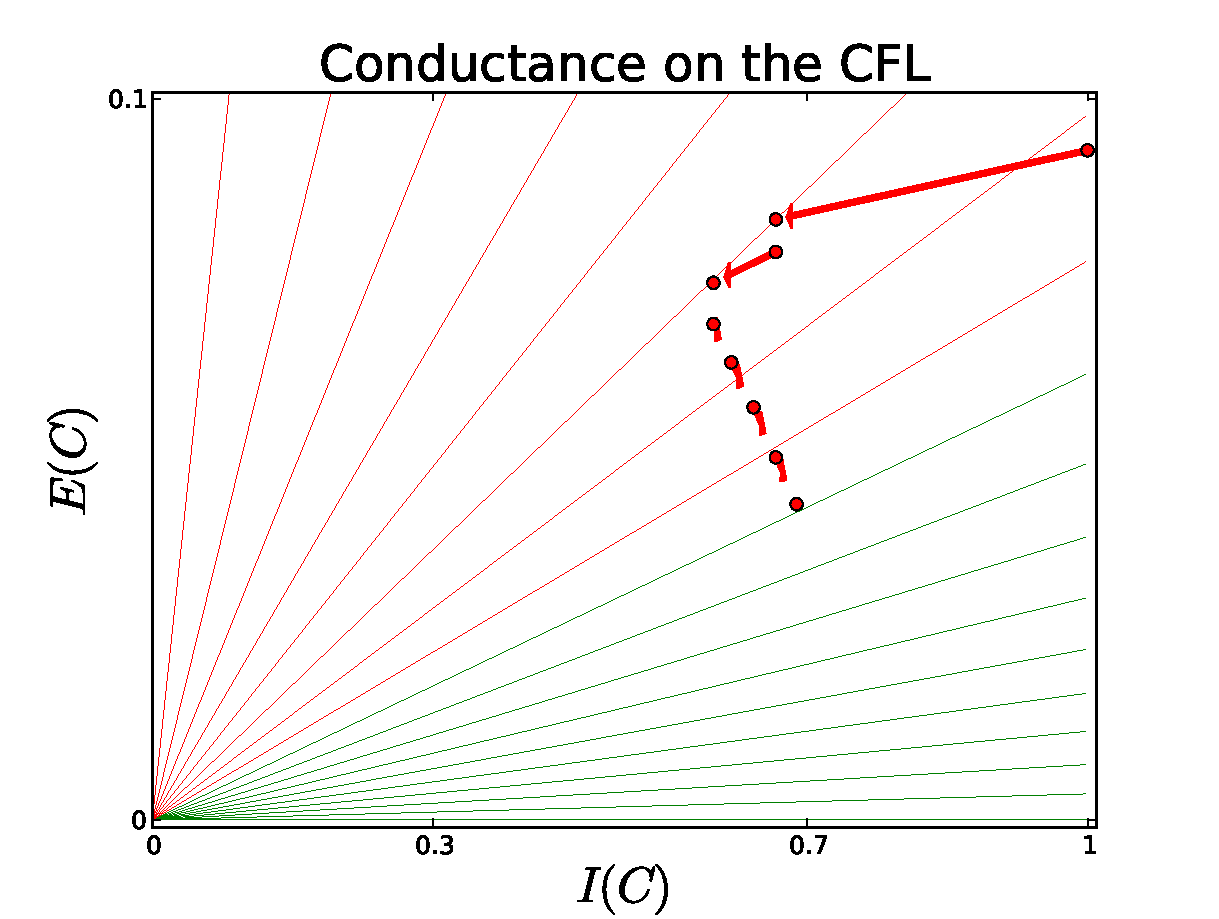
\includegraphics[width=3in]{Figures/football_conductance}
\caption{{\it Conductance is optimized at $E=0$.}The inclusion of level sets makes the movement of conductance across the $I,E$ plane more comprehensible.  The more level sets conductance crosses to make it towards $E=0$, the better the conductance value of the communities is.}
\label{fig_conductance_karate}
\end{figure}

The last parameter that must be taken into account is $k$, the proportion of the graph covered by the community.  Now we fix the $I, E$ ratio and observe how changes in $|C| = k |V|$ affect conductance.  The conclusion,   If the expansion of the community is greatly affected by $k$, then our previous analysis will yield to conductance favoring the largest possible community as demonstrated in {\it Fig. \ref{fig_conductance_a}}.  This affect can be seen in the change of $C_1$ to $C_2$ in the plotted paths in {\it Fig. \ref{fig_conductance_karate}}, as the relative size change of adding just one node is large.

That conductance favors large disconnected communities, even with low internal density, is experimentally confirmed by [].  However, as long as the community is of medium size and has a much larger $I(C)$ value than $E(C)$ conductance will make improvements that correspond to our intuition that an ideal community is internal dense and externally sparse.

\begin{figure}[!h]
\centering
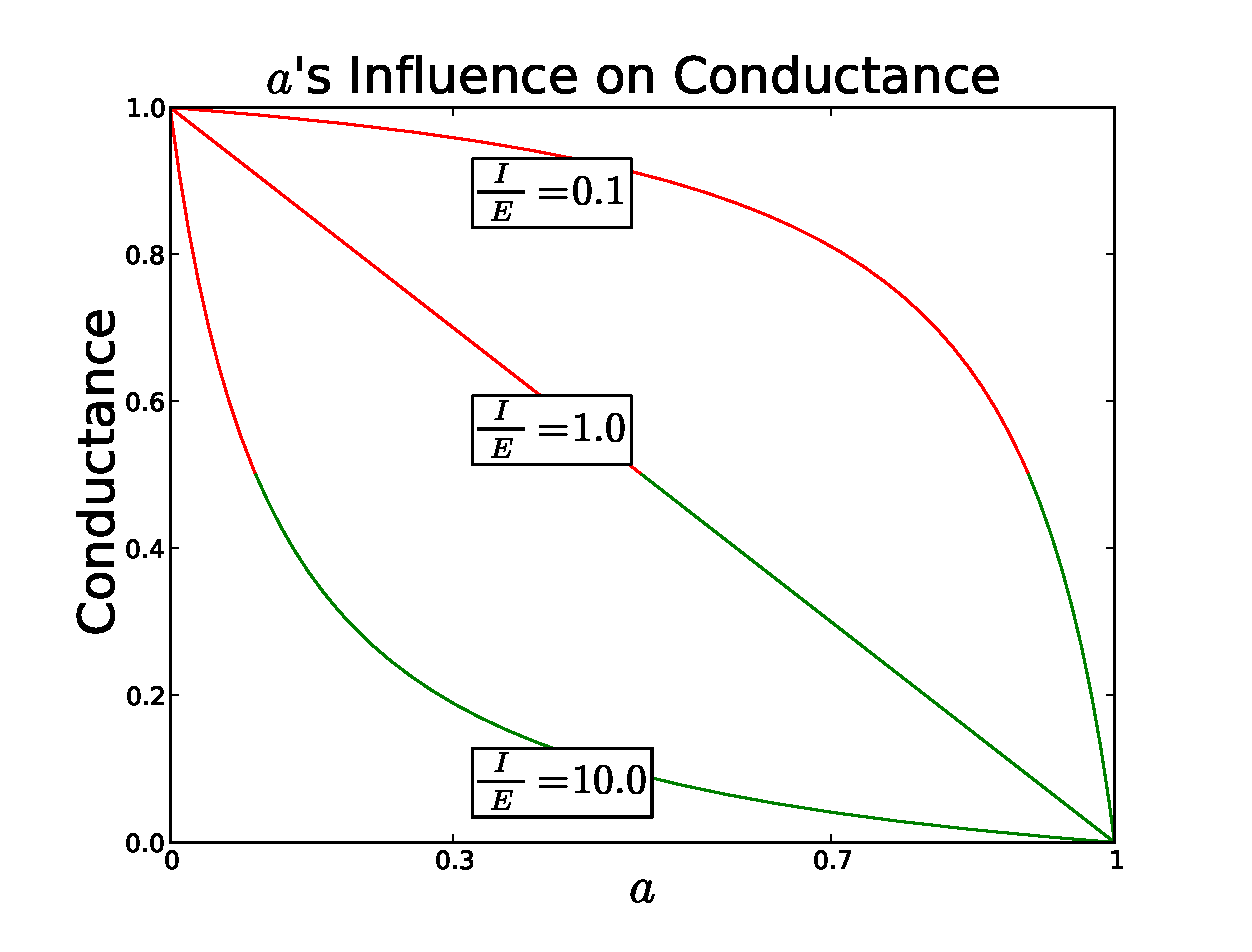
\includegraphics[width=3in]{Figures/Conductance_a}
\caption{{\it Conductance is optimized at $0$.}  The affect the size of the community has on {\sc Conductance}.  Notice that the worst values of conductance correspond to small communities, irregardless of the $I,E$ quality of the community.  Similarly, the best conductance values correspond to the largest communities, irregardless of the internal and external density.}
\label{fig_conductance_a}
\end{figure}

\subsection{Cut Ratio, Edge Cuts, and Expansion}

Similarly as for conductance, showing the level sets of cut ratio, edge cuts, and expansion across the $I,E$ plane reveals the $I,E$ values of the communities that optimize these metrics.  While, the three metrics have different definitions, their level sets are visually identical only with different values.  The level sets are horizontal lines, whose metric's are optimized by improvements in $E(C)$, irregardless of $I(C)$.  Accordingly, the node that has the greatest improvement in $E(C)$ is the same for all three metrics, and each metric results in the same path through the $I,E$ plane.

\begin{figure}[!h]
\centering
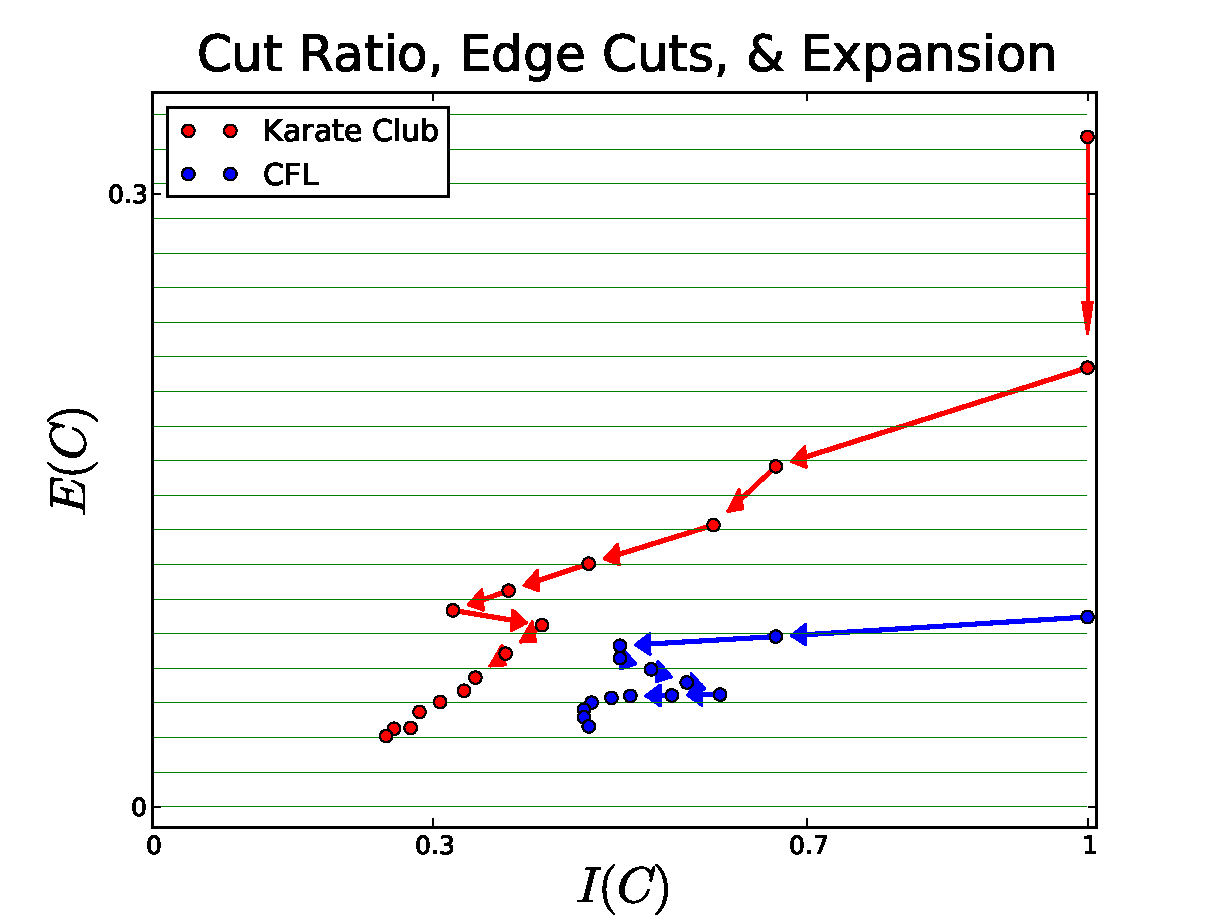
\includegraphics[width=3in]{Figures/cuts_expansion}
\caption{{\it Metrics optimized at $E(C) = 0$.}  Level sets show how cut ratio, edge cuts, and expansion evaluate the $I,E$ plane.  The path corresponds to the $I,E$ values of communities expanded to optimize all three metrics.  Because the level sets are the same, all three metrics produce the same path of optimizing communities in the Karate Club and CFL data sets.}
\label{fig_cuts_expansion}
\end{figure}


Though it does not make a difference in our examples, the difference between these metrics is their treatment of $a$.  Cut ratio is unresponsive to changes in the size of the community, while expansion linearly discount against larger communities.  Edge cuts heavily favors very large or very small communities.  See {\it Fig. \ref{fig_cuts_expansion_a}}

\begin{figure}[!h]
\centering
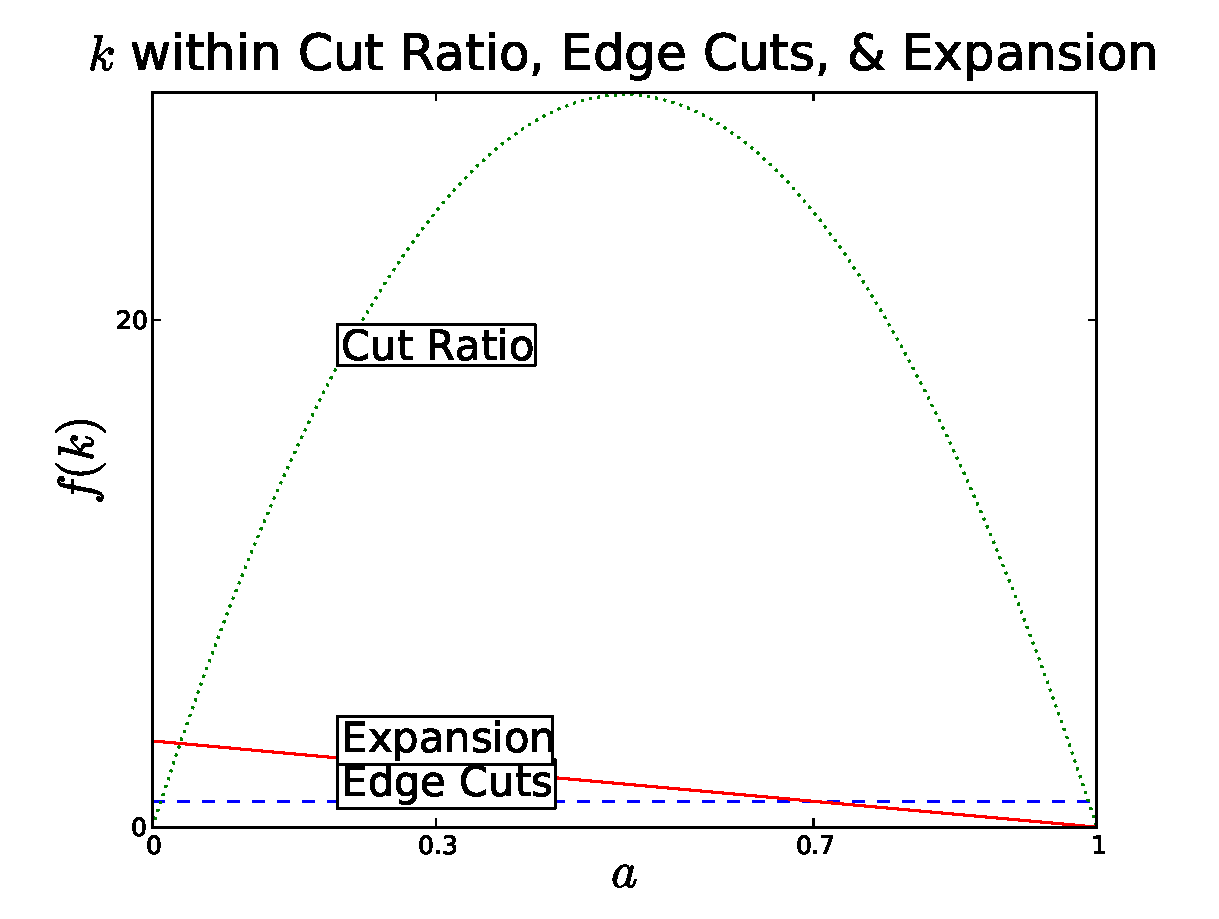
\includegraphics[width=3in]{Figures/cee_k}
\caption{Given a fixed $E(C)$, $f(k)$ is the constant multiple within each of the metrics, that incorporates a factor according to the size of $|C| = k|V$.  These values are specific for the size of communities within the Karate Club.}
\label{fig_cuts_expansion_a}
\end{figure}

\subsection{Internal Density}
On the polar extreme of cut ratio, edge cuts, and expansion, is internal density.  Internal density is a function of internal density and is unresponsive to changes in the the external density.  We do not include indepth analysis, but rather a summary.  The level sets of internal density are vertical lines in the $I,E$ plane.  The paths produced by the greedy algorithm grow out the original community to the largest clique it can find, as the internal density of two connected notes is already maximal.  Any clique is an optimization of internal density, irregardless of external connectivity.

\subsection{Volume}
A metric that takes both internal and external density into account is volume.  The next conclusion is not apparent just from the equation parameterized in terms of internal and external density.  However, observing the level sets of volume reveal that the optimal community is at $(I, E) = (0, 0)$ and volume as a metric is optimal for communities with low external density and low internal density.  Apart from communities of disconnected nodes, volume can best be optimized by a community encompassing the entire graph.  Volume directly contradicts our intuition that communities should have good internal connectivity.
\begin{figure}[!h]
\centering
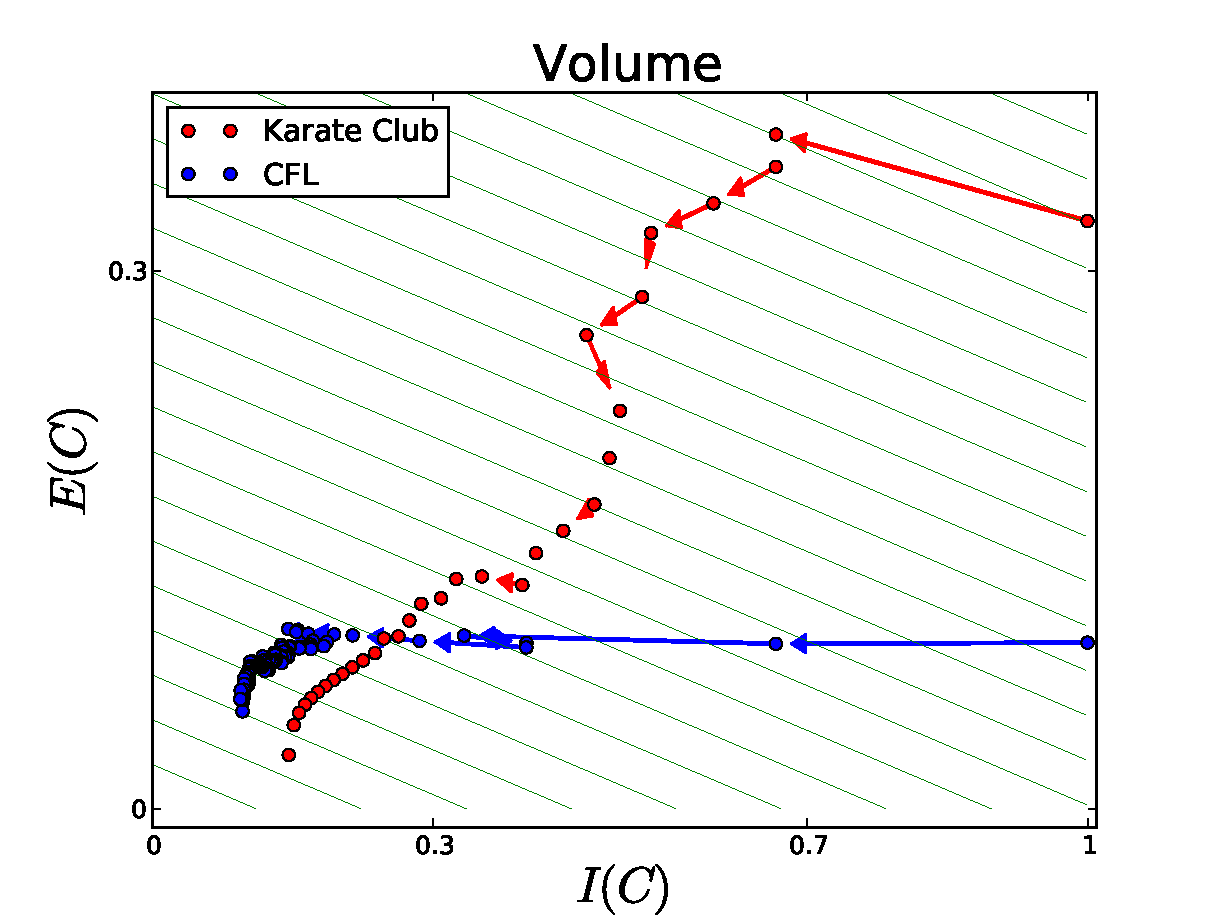
\includegraphics[width=3in]{Figures/volume}
\caption{Given a fixed $E(C)$, $f(a)$ is the constant multiple within each of the metrics, that incorporates a factor according to the size of $|C| = k|V|$.  These values are specific for the size of communities within the Karate Club.}
\label{fig_volume}
\end{figure}

\subsection{Linearity}

We maintain that the variables of internal and external density incorporate our full intuition of communities, metrics are just a matter of balancing between the two.  We have shown how previous metrics single communities balance the two or select one to optimize for.  We propose a linear metric that transparently balances between the two variables.
\begin{definition}[Linearity]
 Our metric for single communities:
  \begin{align}
   \text{\sc Linearity} = M_L(C) &= a I(C) - b E(C)
  \end{align}
\end{definition}
Many metrics incorporated the size of the community into their weighting.  Indeed, it is more significant for a large community to gain nearly the same internal density as small community.  Accordingly, there is a generalization of {\sc Linearity} that can account for any desired weighting between internal and external density, with weighting for any size of community.
\begin{definition}[General Metric]
 Our metric for single communities in its greatest generality:
  \begin{align}
   \text{\sc General} = M_G(C) &= \sum\limits_{i = 0} f_i(C) I(C)^i - g_i(C) E(C)^i
  \end{align}
\end{definition}
Where $f_i$ and $g_i$ can be any function of the size of a community.

Linearity behaves similarly to conductance, when conductance is in a region of the $I,E$ plane where there is a fair balance between improvements of $I$ and $E$.  Unlike conductance though, linearity does not have a critical point in the $I,E$ plane, where the balance is shifted towards only favoring improvements in $E$.  The result is that with the same initial seeds in the Karate Club and CFL, linearity follows the same path as conductance for the first few expansions and stops, rather than engulfing the network.

\subsection{Optimal Communities}

To conclude our analysis of metrics for the Karate Club and the CFL networks we present the optimal communities within the network according to each metric.  For the Karate Club the optimal communities are:
\begin{tabular}{|c | c  c  |}
 \hline Metric & Optimal $C$ & $(I(C), E(C))$ \\ \hline
{\sc Conductance} & $G$& $(0.14, 0)$\\ \hline
{\sc Cut Ratio}  & $G$ & $(0.14, 0)$\\ \hline
{\sc Edge Cuts}  & $G$& $(0.14, 0)$ \\ \hline
{\sc Expansion}  & $G$&$(0.14, 0)$ \\ \hline
{\sc Internal Density}  & $\{u,v\} | w(u,v) = 1$ & $(1, x)$ \\ \hline
{\sc Linearity}  & clique of $3$ nodes & $(1, 0.04)$ \\ \hline
{\sc Volume}  & $G$& $(0.14, 0)$ \\ \hline
\end{tabular}
The same trend holds for the CFL network, except with {\sc Linearity} returning a set of different nodes according to $a$ and $b$ in the metric.

\section{Metrics for Sets of Communities}

Our original parameterization of internal and external density can not be directly applied to a set of communities, $S = \{C_1, C_2, \dots C_n\}$.  Though if we follow the same logic we will arrive at a similar parameterization.  An ideal set of communities are cliques such that every edge is within some community.  In addition, the community description of the network should not have an exponential number of communities, but rather some concise set of communities.  Hence an ideal set of communities has three parameters.  Internal density is a representation of how close the set of communities is to being a set of cliques.  External density is a representation of how close the set of communities are to covering all edges in the graph.  Size of the set of communities is a representation of how concise the set of communities are.  We pick the following representations, but note that different representations do not yield different conclusions in the following sections.

\begin{definition}[Internal Density for  a Set of Communities]
 \begin{align*}
    I(S) &=  \sum_{C \in S} \frac{\sum_{u \in C}\sum_{v \in C} w(u,v)}{\sum_{C \in S} |C|(|C| - 1)}
 \end{align*}
\end{definition}

\begin{definition}[External Density for  a Set of Communities]
 \begin{align*}
  E(S) &= \frac{\sum_{(u,v) \in \text{\sc ext\_edges}}w(u,v)} {\sum_{u \in V}\sum_{v \in V} w(u,v) }
 \end{align*}
\end{definition}

\begin{definition}[Conciseness for  a Set of Communities]
 \begin{align*}
  \text{\sc Conciseness}(S) &= |S|
 \end{align*}
\end{definition}

To date we do not know of any previous metrics that have a closed form parameterization in terms of $I(S)$, $E(S)$, and $|S|$.  We release a linear metric pertaining to these parameters in a later section.

\begin{definition}[Ideal Set of Communities]
 A set of communities, $S$, is ideal if it is a set of cliques that cover the graph in the fewest necessary communities:
  \begin{align*}
   I(S) &= 1 \\
   E(S) &= 0 \\
  |S| &= 1. 
  \end{align*}
\end{definition}

\subsection{Modularity}

Modularity is a partitioning of the network, and each partition is deemed a community.  For each module its modularity is the difference of the existing internal edges and expected number of internal edges, had the graph been random, with the same distribution of node degrees.  The total modularity is then the sum of the modularity of each partition.  Modularity was developed by [] and has found wide spread use due to the fast algorithms for maximizing modularity \cite{modularity}.  In particular, the use of dendograms in the Louvain Algorithm \cite{louvain} runs in minutes for large networks.

There is not a closed form parameterization of modularity in terms of our definitions of $I(S)$, $E(S)$, and $|S|$.  But we find $I(S)$ and $E(S)$ to be intuitive enough to provide the space in which to analyze metrics of sets of communities.

Still, we would like to be able to use level sets for some visual explanation of how modularity behaves with regard to some internal and external density.  The parameterization of modularity we can provide is in terms of $I(C)$ and $E(C)$ for single communities.  If we allow, $p=\frac{|C|(|C|-1)}{2L}$ and $q=\frac{|C|(|V|-|C|)}{2L}$ to be constants:
\begin{align}
 \text{\sc Modularity}(S) = \sum_{C \in S} p I(C) - \left(p I(C) + q E(C)\right)^2.
\end{align}
\begin{figure}[!h]
\centering
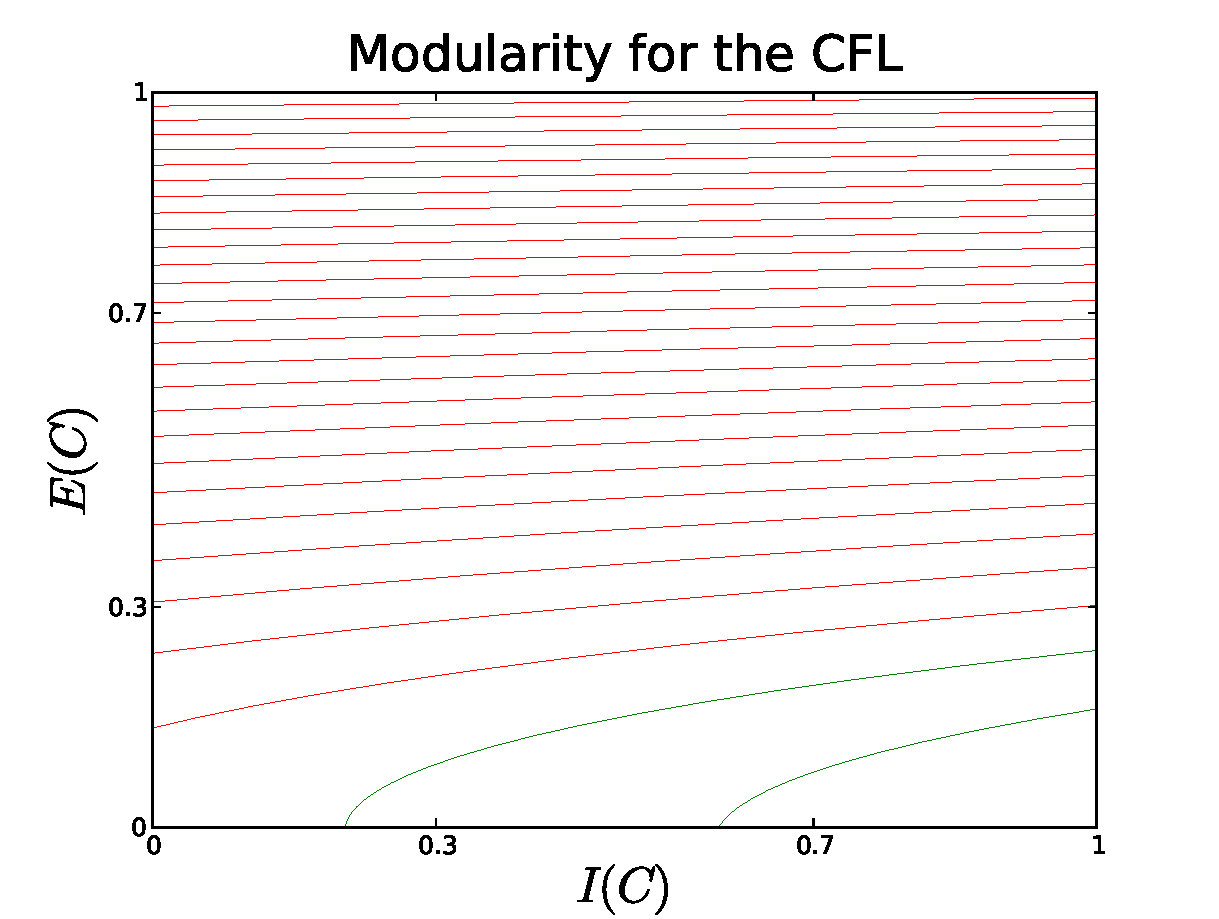
\includegraphics[width=3in]{Figures/cfl_mod_ls}
\caption{The level sets of how {\sc Modularity} treats the $I(C)$, $E(C)$ space for one community of size 9 in the CFL.  Note the sharp transition from a region that heavily favors improvements in external density to a region that heavily favors improvements in internal density($E(C) < 0.1$).}
\label{fig_f_cfl}
\end{figure}
We can draw loose conclusions from this parameterization.  The first check is that a set of disjoint cliques are the only communities that optimize modularity.  There are no counter intuitive communities that optimize modularity.  Overall, modularity is a two part optimization.  For seed communities, in the case of modularity individual nodes, the typical initial values are high in external density.  When $E(C)$ is high it is the dominating term and the optimization is to decrease $E(C)$ as quickly as possible.  Once, external density is not the dominating term the optimization is then center around trying to improve $I(C)$.  The transition between these two phases of optimization is sudden as attested by the level sets.

We would like to recommend modularity should be designed to optimize for improvements in internal density first to find the dense cores of communities and then optimize over external density to cover more of the graph.  The reasoning is that improvements in external density can be made at any time by increasing the size of communities.  However, improvements in internal density can only be made while the communities are small and closer to cliques.


\subsection{Linearity for Sets of Communities}

We now present a linear metric for sets of communities with regard to $I(S)$, $E(S)$, and $|S|$.  It follows the same intuition of creating the linear metric for a single community.  The ideal community is located at $(I(S), E(S), |S|) = (1, 0, 0)$ and accordingly the level sets are parallel planes emanating from around the ideal community.  Hence, the linearity of the metric.  How to balance between improvements in each of the parameters is set by the user.
\begin{definition}[Linearity]
 Our metric for a set of communities:
  \begin{align*}
   \text{\sc Linearity}(S) &= a I(S) - b E(S) - c |S|,
  \end{align*}
where $a,b,c \geq 0$.
\end{definition}
Depending on the application, communities of certain characteristics may be desired.  Communities of size smaller than a certain size may be desired to be penalized or trade offs between improvements in $E(S)$ and $I(S)$ may depend on existing values.  A general form of this equation is available.
\begin{definition}[General Metric]
 Our metric for single communities in its greatest generality:
  \begin{align*}
   \text{\sc General} (S) &= \sum\limits_{i = 0} f_i(S) I(S)^i - g_i(S) E(S)^i - h_i |S|^i
  \end{align*}
\end{definition}



\subsection{Performance}
We now empirically compare {\sc Linearity}$(S)$ and {\sc Modularity}$(S)$.  Theoretically, modularity is expected to begin with trades of large improvements in external density, $E(S)$, for large losses of internal density, $I(S)$.  Once the portion of graph is reached where internal density is more highly favored modularity will be maximized, as further improvements to internal density will not exist.  Theoretically, linearity is expected to make the same trade off at every stage producing a nearly linear path through the $I(S)$, $E(S)$ space.

The compute the sets of communities that maximize each metric we use the Louvain algorithm[].  The algorithm does not need to be modified to maximize modularity.  We easily adapt Louvain's algorithm to maximize linearity for sets of communities.  Once we run the adapted Louvain algorithm for maximizing linearity we can further maximize linearity by expanding the partitions into overlapping communities.  We note that no expansion making a full community a subset of another community will be optimal.  Hence, we can use a greedy algorithm to expand the partitions produced by the Louvain algorithm.  We expand each community to overlap neighboring communities if the metric is improved by doing so.  We have tested running expansion off of the partition given by maximizing modularity and find that the following results are still optimized by using the partition given by maximizing linearity.  The following figures{\it Fig. \ref{fig_k_cfl}}, {\it Fig.\ref{fig_astro}}, and {\it Fig} show how the partitions produced by each metric being optimized are quickly divergent.

Maximizing the metrics involves a process of starting with set of communities, finding the maximal beneficial union of communities and iterating.  Once a beneficial union is found the set of communities changes to reflect this.  For each metric then we can produce a path of $S_1, S_2, \dots$ that represent the intermediary sets of communities chosen by the metric.  We can then plot this path of sets of communities in the $I(S), E(S)$ plane to see how the metric balances between internal and external density for a given network.

\begin{figure}[!h]
\centering
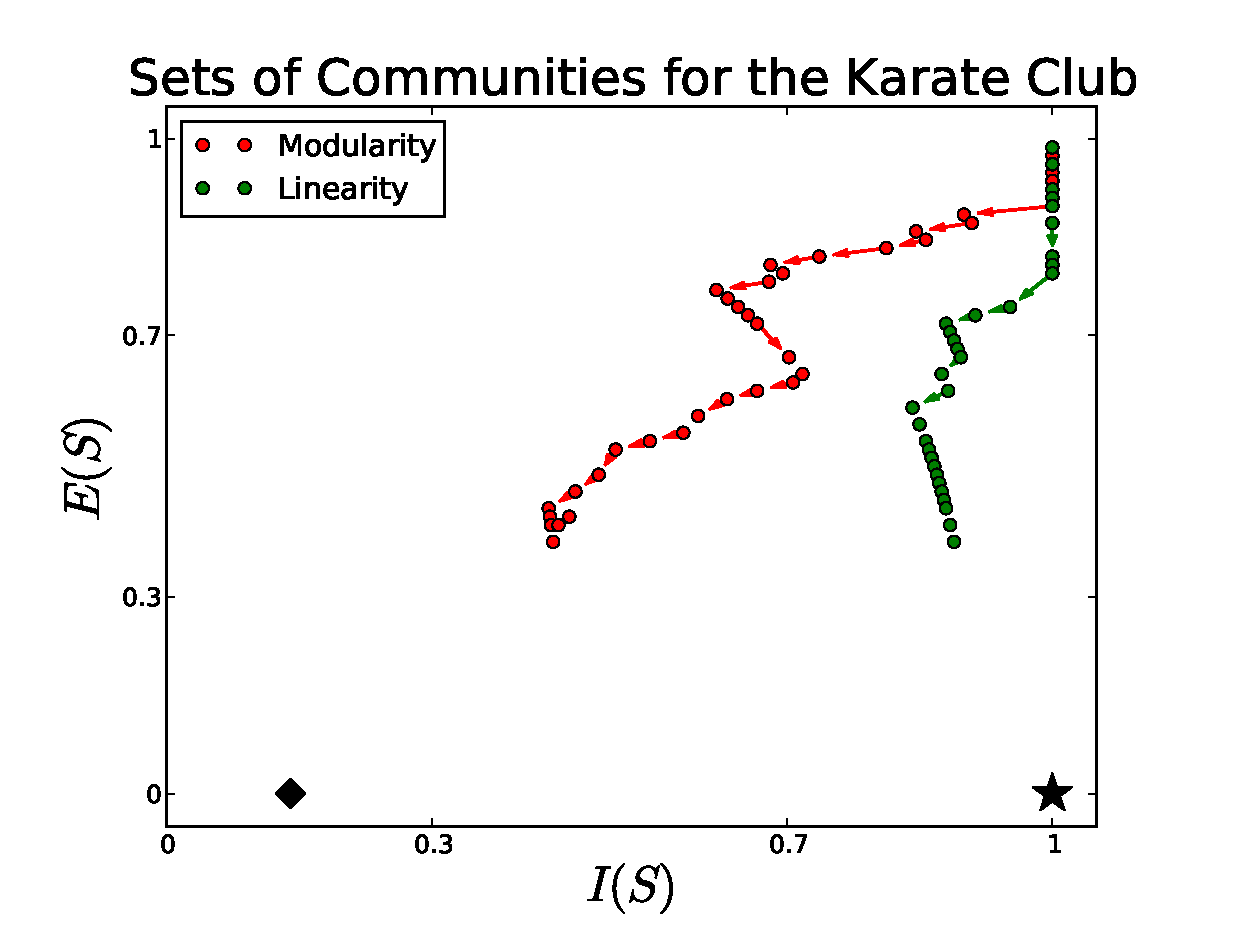
\includegraphics[width=3in]{Figures/Karate_Club_ml}
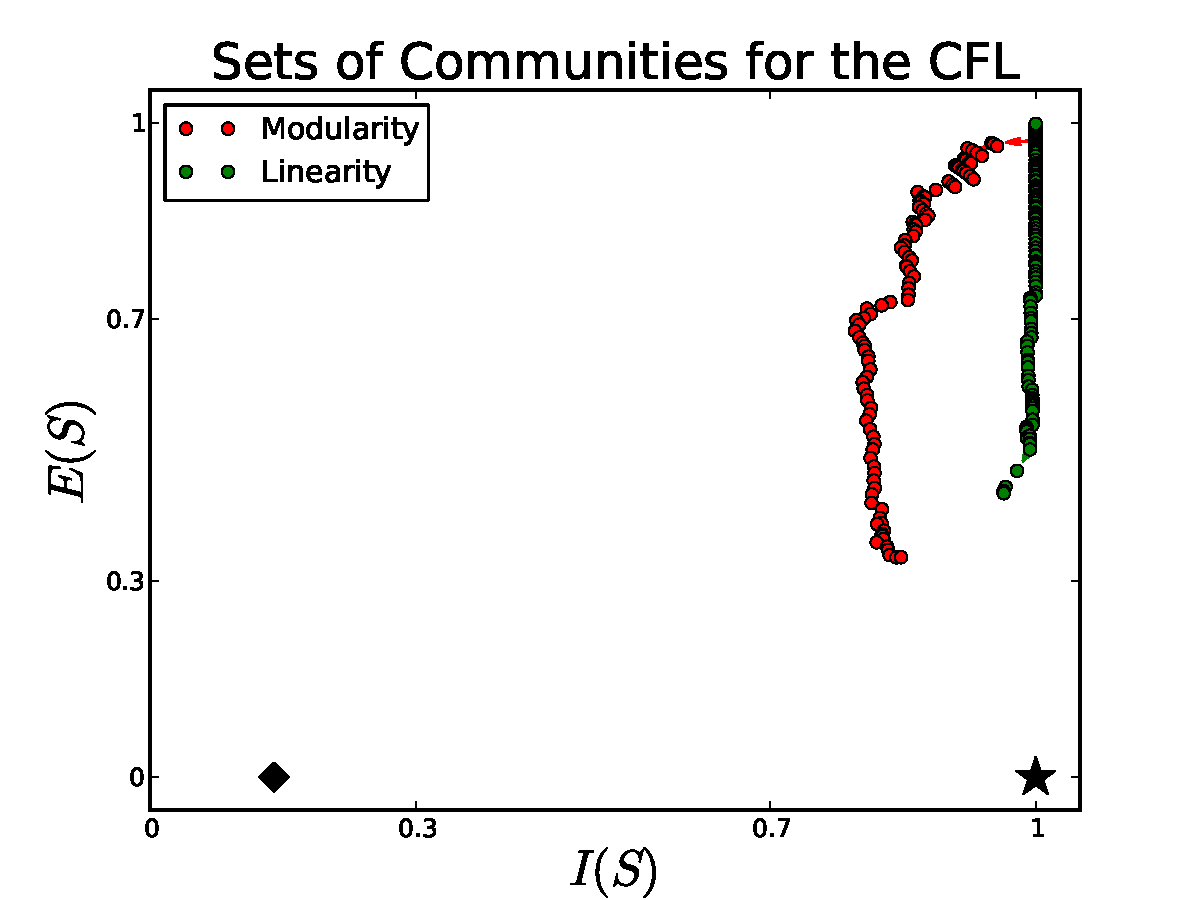
\includegraphics[width=3in]{Figures/CFL_ml}
\caption{The series of sets of communities produced by optimizing modularity and linearity, plotted by their $(I(S), E(S))$ values.  The third parameter not displayed is how many communities are within each set.  Linearity produces 16 and 18 communities for the karate club and the CFL respectively.  Similarly. modularity produces 5 and 13 communities.}
\label{fig_k_cfl}
\end{figure}

\begin{figure}[!h]
\centering
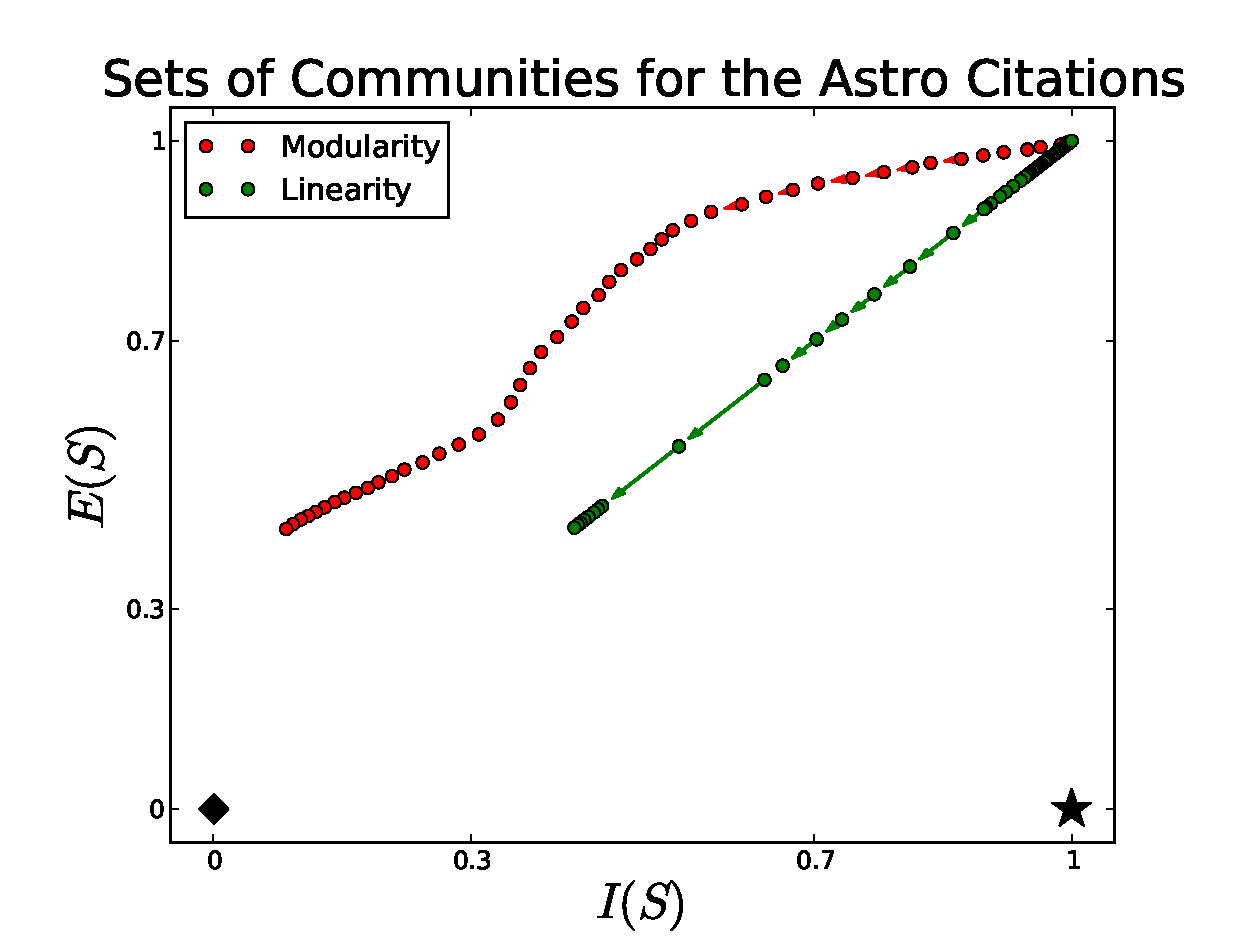
\includegraphics[width=3in]{Figures/astro_ml}
\caption{Using the astrophysics citation network from [], with approximately 19k nodes and 200k edges, we apply the Louvain algorithm for modularity maximization and the adapted Louvain algorithm for linearity maximization.  For the dimension not shown, conciseness, modularity produced 1523 communities and linearity produced 1258 communities.  The points shown for linearity are an evenly spaced sample of changes to the set of communities.  The points shown for modularity are the value of the communities at each stage of the dendogram.
The black star corresponds to the ideal values for a set of communities.  The black diamond corresponds to the value of a community encompassing the entire graph.  Overall, linearity uses slightly fewer communities to have significantly higher internal density with comparable coverage of all edges of the graph.}
\label{fig_astro}
\end{figure}

Because linearity is a direct optimization of parameters internal density, $I(S)$, external density $E(S)$, and conciseness, $|S|$,  it can be modified through $a$, $b$, and $c$ within {\sc Linearity}$(S)$ to always outperform {\sc Modularity}$(S)$ with regard to at least two parameters.  In fact, it is only because of the inclusion of all three parameters that allows {\sc Linearity} to return meaningful results.  Trivial sets of communities exist for optimizing any two of the parameters.  However, linearity exceeds expectations and outperforms in all three parameters for communities for the astrophysics citation network {\it Fig. \ref{fig_astro}}.  If the partition produced by maximizing linearity is compared to the partition produced by maximizing modularity, in terms of modularity it is surprisingly close, considering that they are completely different optimizations with very different $I(S), E(S)$ values.




\section{Conclusion}

The process we have used is straightforward.  When designing a metric of testing the value of a single community or a set of communities, we began by describing the ideal communities.  Once described the properties of the ideal communities could be named.  In a single community's evaluation internal and external density are measured.  A set of communities are evaluated on internal density, coverage of the network, and conciseness of the communities.  Formalizing each of these properties, previous metrics could be analyzed in how they treated these properties.  Visualization of their biasnesses could be seen from producing level sets.  Different treatments of these properties then presented themselves.  In particular, linear combinations of these parameters were revealed and transparently optimized towards the ideal values for internal and external density.

If dense internal structures and sparse external connectivity is desired in single communities, those properties can be directly optimized for with {\sc Linearity}$(C)$.

If dense internal structures, large coverage of the network, and a concise community description are desired, those properties can be directly optimized for with {\sc Linearity}$(S)$.


\subsection{Future Work}

While we have demonstrate a new framework and the metrics produced by an explicit relationship between internal density and external density, we have not fully explored the communities produced by varying that relationship.  To date, we have only used iterative search of $a$, $b$, and $c$ to find an optimal path through the internal and external density spaces.  We have noticed that while there is infinite choice in setting $a$, $b$ and $c$ there are only a few possible paths through the $I$, $E$ space, which has made finding appropriate values for $a$, $b$ and $c$ quick.  We have not formalized this property or explored what it is about the structure of graphs that causes it.

The algorithm used to optimize linearity is a basic and fast algorithm, not designed around optimizing linearity.  There is perhaps some gain to finding an algorithm that interweaves the step of finding larger communities and overlapping them.  We have not tried the overlapping algorithm for modularity from [Ahn, etal ].


More citations to follow.

Application to larger networks.

% trigger a \newpage just before the given reference
% number - used to balance the columns on the last page
% adjust value as needed - may need to be readjusted if
% the document is modified later
%\IEEEtriggeratref{8}
% The "triggered" command can be changed if desired:
%\IEEEtriggercmd{\enlargethispage{-5in}}

% references section

% can use a bibliography generated by BibTeX as a .bbl file
% BibTeX documentation can be easily obtained at:
% http://www.ctan.org/tex-archive/biblio/bibtex/contrib/doc/
% The IEEEtran BibTeX style support page is at:
% http://www.michaelshell.org/tex/ieeetran/bibtex/
%\bibliographystyle{IEEEtran}
% argument is your BibTeX string definitions and bibliography database(s)
%\bibliography{IEEEabrv,../bib/paper}
%
% <OR> manually copy in the resultant .bbl file
% set second argument of \begin to the number of references
% (used to reserve space for the reference number labels box)
\begin{thebibliography}{1}

\bibitem{leskovec:empirical}
J.~Leskovec, K.~Lang, and M.~Mahoney, \emph{Empirical Comparison of Algorithms for Network Community Detection}, { ACM WWW International conference on World Wide Web (WWW)}, 2010.

\bibitem{louvain}
V.~Blondel, J.~Guillaume, R.~Lambiotte, and E.~Lefebvre, \emph{Fast Unfolding of Communities in Large Networks}, {Journal of Statistical Mechanics: Theory and Experiment}, 2008.

\bibitem{modularity}
M.~Newman, \emph{Modularity and community structure in networks}, {PNAS}, June 6, 2006 vol.103 no.23 8577-8582.

\bibitem{conductance}
B.~Bollobas, \emph{Modern Graph Theory}, {Springer Verlag}, New York, USA 1998.

\bibitem{clauset}
A.~Clauset, M.~Newman, and C.~Moore, \emph{Finding community structure in very large networks}, {Physics Review} E 70, 066111, 2004.

\end{thebibliography}



\end{document}